\documentclass[convert]{standalone}

\usepackage{tikz}
\usepackage{graphicx}
\pagestyle{empty}

% INT_AY21_L16_Fig01_FBD.png

\begin{document}
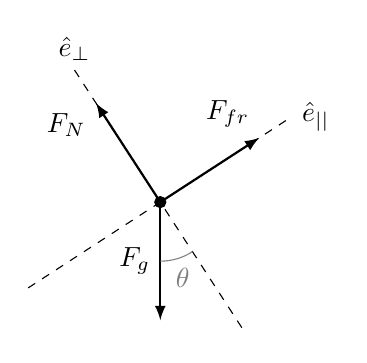
\begin{tikzpicture}[> = latex]

	% Define the ramp angle
	
	\def\Q{33}
	
	% The dot
	
	\filldraw (0, 0) circle (2 pt);
	
	% Coordinate axes
	
	\draw [dashed] (180 + \Q : 2) -- (\Q : 2) node [right] {${\hat e}_{||}$};
	\draw [dashed] (90 + \Q : 2) node [above] {${\hat e}_\perp$} -- (270 + \Q : 2);
	
	% Three forces on child
	
	\begin{scope}[->, thick]
	
		\draw (0, 0) -- (90 + \Q: 1.5) node [below left] {$F_N$};
		\draw (0, 0) -- node [left] {$F_g$} (270 : 1.5);
		\draw (0, 0) -- (\Q : 1.5) node [above left] {$F_{fr}$};
		
	\end{scope}
	
	% Angle indicator for force F_g
	
	\draw [gray] (0, -0.75) arc (270 : 270 + \Q: 0.75);
	\node [gray] at ({270 + 0.5 * \Q} : 1) {$\theta$};
		
\end{tikzpicture}
\end{document}